% !TEX TS-program = pdflatex
% !TEX encoding = UTF-8 Unicode

\documentclass[a4paper, titlepage=false, parskip=full-, 10pt]{scrartcl}

\usepackage[utf8]{inputenc}
\usepackage[T1]{fontenc}
\usepackage[english, ngerman]{babel}
\usepackage{babelbib}
\usepackage{hyperref}
\usepackage{listings}
\usepackage{framed}
\usepackage{color}
\usepackage{graphicx}
\usepackage[normalem]{ulem}
\usepackage{cancel}
\usepackage{amsmath}
\usepackage{amssymb}
\usepackage{amsthm}
\usepackage{algorithm}
\usepackage{algorithmic}
\usepackage{geometry}
\usepackage{subfigure}
\geometry{a4paper, top=20mm, left=35mm, right=25mm, bottom=40mm}

\newcounter{tasknbr}
\setcounter{tasknbr}{1}
\newenvironment{task}[1]{{\bf Aufgabe \arabic {tasknbr}\stepcounter{tasknbr}} (#1):\begin{enumerate}}{\end{enumerate}}
\newcommand{\subtask}[1]{\item[#1)]}

% Listings -----------------------------------------------------------------------------
\definecolor{red}{rgb}{.8,.1,.2}
\definecolor{blue}{rgb}{.2,.3,.7}
\definecolor{lightyellow}{rgb}{1.,1.,.97}
\definecolor{gray}{rgb}{.7,.7,.7}
\definecolor{darkgreen}{rgb}{0,.5,.1}
\definecolor{darkyellow}{rgb}{1.,.7,.3}
\lstloadlanguages{C++,[Objective]C,Java}
\lstset{
escapeinside={§§}{§§},
basicstyle=\ttfamily\footnotesize\mdseries,
columns=fullflexible,
keywordstyle=\bfseries\color{blue},
commentstyle=\color{darkgreen},      
stringstyle=\color{red},
numbers=left,
numberstyle=\ttfamily\scriptsize\color{gray},
breaklines=true,
showstringspaces=false,
tabsize=4,
captionpos=b,
float=htb,
frame=tb,
frameshape={RYR}{y}{y}{RYR},
rulecolor=\color{black},
xleftmargin=15pt,
xrightmargin=4pt,
aboveskip=\bigskipamount,
belowskip=\bigskipamount,
backgroundcolor=\color{lightyellow},
extendedchars=true,
belowcaptionskip=15pt}

%% Enter current values here: %%
\newcommand{\lecture}{Computer Vision WS15/16}
\newcommand{\tutor}{}
\newcommand{\assignmentnbr}{5}
\newcommand{\students}{Julius Auer}
%%-------------------------------------%%

\begin{document}  
{\small \textsl{\lecture \hfill \tutor}}
\hrule
\begin{center}
\textbf{Übungsblatt \assignmentnbr}\\
[\bigskipamount]
{\small \students}
\end{center}
\hrule

\begin{task}{Histogram of Oriented Gradients}
\item[]
\begin{itemize}
\item\emph{implementiere eine Funktion zur Extraktion eines Winkelhistogramms wie in der Vorlesung beschrieben (für Zellen der Größe 8 x 8 Pixel)}
\item\emph{benutze diese Funktion für die Extraktion des HOGs für die Organisationsebenen Blöcke und ROIs}
\item\emph{implementiere eine Funktion, die, gegeben ein Winkelhistogramm, die Hauptkantenrichtung in einem Block als weiße Linie auf schwarzem Hintergrund darstellt}
\item\emph{benutze diese Funktion, um das Eingabebild person.png als Mosaik aus diesen Hauptkantenrichtungskacheln darzustellen (Abgabe 1.1)}
\end{itemize}

Die Gradienten werden naiv mit den x,y-Sobel-Filtern generiert. Aus den Farbkanälen wird der dominante gewählt. Für diesen einfachen Fall schien es nicht erforderlich noch NMS, Smoothing oder andere Optimierungen anzuwenden. Abbildung \ref{fig:1} zeigt das Gradientenbild (als HSV, mit H: Gradienten-Richtung (9 diskrete Werte), S: 1, V: Gradienten-Magnitude).

\begin{figure}[!htpb]
\centering
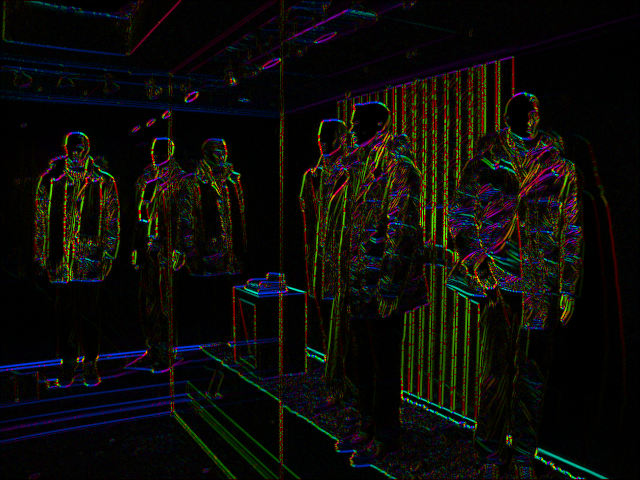
\includegraphics[width=0.48\linewidth]{captures/gradients}
\caption{Gradientenbild}
\label{fig:1}
\end{figure}

Die Zellgröße beträgt $8\times 8$ Pixel und die Blockgröße $2\times 2$ Zellen. Die Normierung in den Blöcken erfolgt naiv (linear). Abbildung \ref{fig:2} zeigt die Richtungen der dominierenden Gradienten für Zellen und Blöcke. Da Vorzeichen nicht betrachtet werden genügen Linien (keine Pfeile). Als Teilmenge vom abgebildeten \emph{people.png} ist auch - wie gefordert - \emph{person.png} zu sehen ;)

\begin{figure}[!htpb]
\centering
\subfigure[Zellen]{
  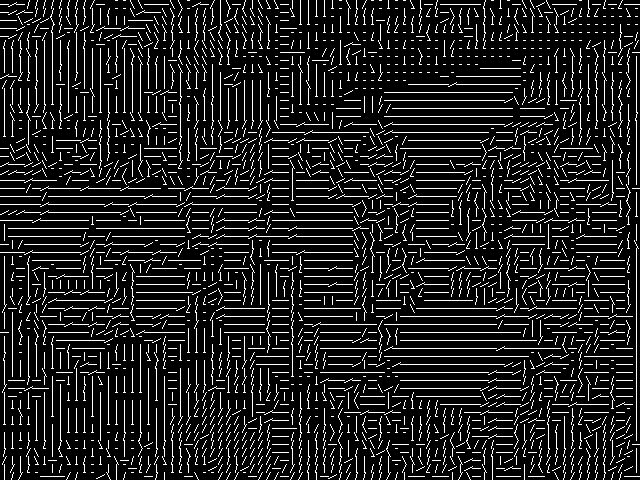
\includegraphics[width=0.48\linewidth]{captures/cells}
}
\subfigure[Blöcke]{
  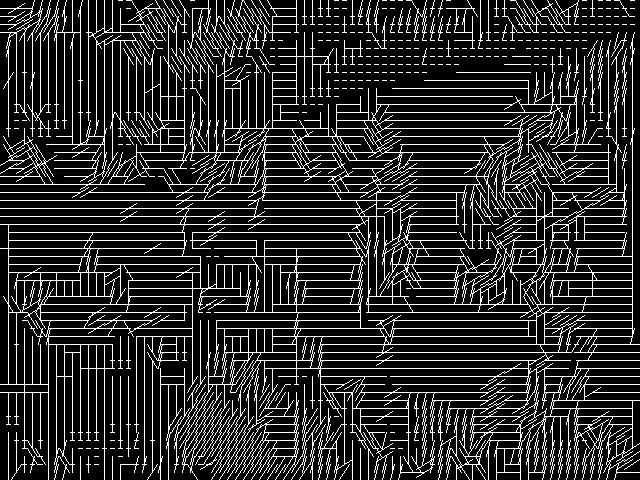
\includegraphics[width=0.48\linewidth]{captures/blocks}
}
\caption{Mosaik aus Hauptkantenrichtungen}
\label{fig:2}
\end{figure}

\newpage
\begin{itemize}
\item\emph{implementiere die Suche nach Personen in beliebig großen Eingabebildern. Nimm dazu eine Suchfenstergröße von 144 x 384 Pixeln an. Suche in den Bildern people.png und people2.png nach Personen. Nutze für die Entscheidung, ob ein ROI eine Person enthält die Vorlage person.png. Stelle bei positivem Ergebnis das jeweilige ROI als Overlay auf dem Bild dar (Abgabe 1.2 und 1.3).}
\end{itemize}

Als einfache Lösung wurde naiv die ROI mit dem kleinsten quadratischen Fehler gewählt. Das Ergebnis zeigt Abbildung \ref{fig:3}.

\begin{figure}[!htpb]
\centering
\subfigure[people]{
  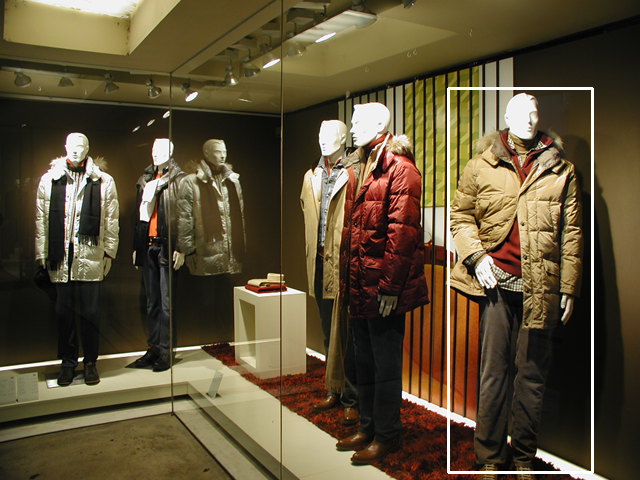
\includegraphics[width=0.48\linewidth]{captures/people1}
}
\subfigure[people2]{
  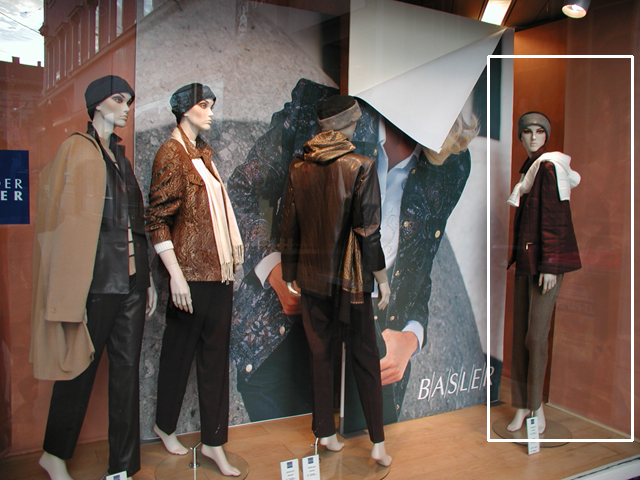
\includegraphics[width=0.48\linewidth]{captures/people2}
}
\caption{ROI mit kleinstem Fehler}
\label{fig:3}
\end{figure}

\newpage
Zeichnet man ein paar ROIs mehr (Abbildung \ref{fig:3}), wird deutlich, dass auch andere Personen vernünftig erkannt werden. Man könnte hier mit einem etwas ambitionierterem Verfahren auch eine Menge von Personen extrahieren. 

\begin{figure}[!htpb]
\centering
\subfigure[people]{
  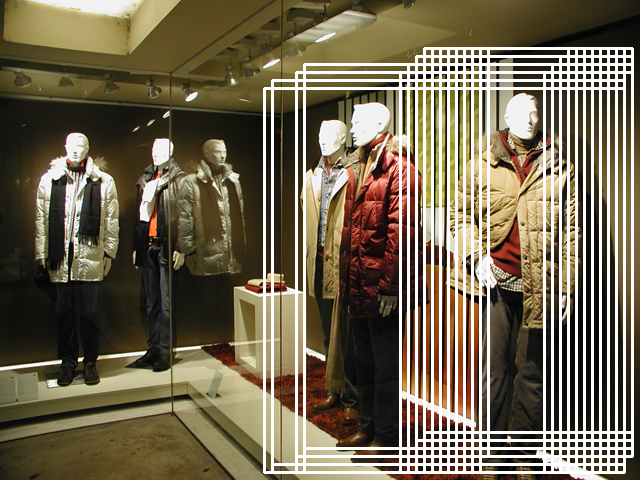
\includegraphics[width=0.48\linewidth]{captures/people1-2}
}
\subfigure[people2]{
  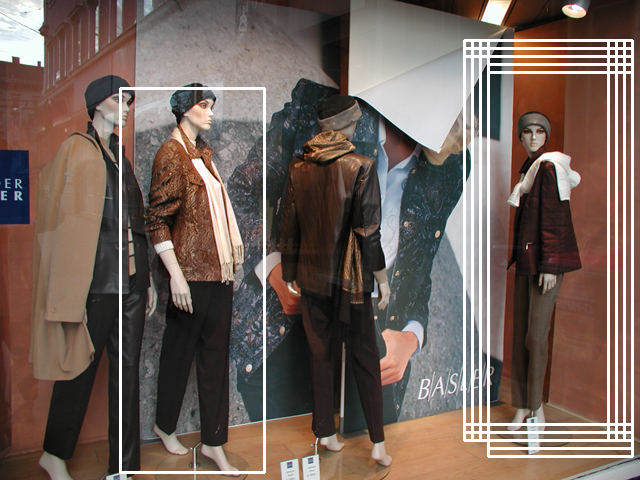
\includegraphics[width=0.48\linewidth]{captures/people2-2}
}
\caption{ROIs mit kleinem Fehler}
\label{fig:3}
\end{figure}
\end{task}
\end{document}
